% Note: this problem is very similar to Problem03 but doesn't require sketching asymptotes.

Use root locus analysis to answer the questions about the following feedback control system.

\begin{center}
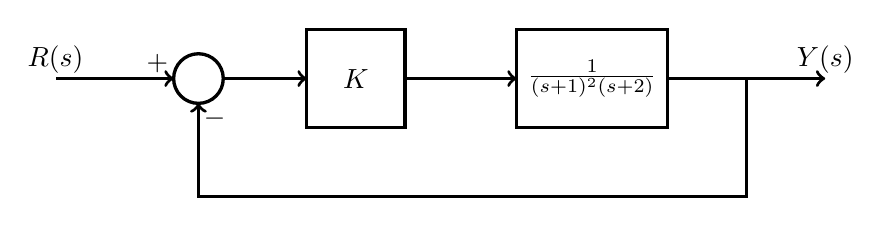
\begin{tikzpicture}[scale=1,inner sep=0pt,outer sep=0pt,very thick,
sysblock/.style={draw,rectangle,inner sep=4pt,minimum width=1.25cm,minimum height=1.25cm,very thick}]

\draw (-2,0) node[draw,circle] (sum1) {$\rule{0pt}{18pt}$};
\draw (0,0) node[sysblock] (K)  {$K$};
\draw (3,0) node[sysblock] (G) {$\frac{1}{(s+1)^2(s+2)}$};
\draw[<-] (sum1.180) node[above left=2pt] {$+$} -- ++(-1.5,0) node[above=2pt] {$R(s)$};
\draw[->] (sum1.0) -- (K.180);
\draw[->] (K.0) -- (G.180);
\draw[->] (G.0) --  ++(2,0) node[above=2pt] {$Y(s)$};
\draw[->] (G.0) -- ++(1,0) -- ++(0,-1.5) -| (sum1.-90) node[below right=2pt] {$-$};
\end{tikzpicture}
\end{center}

\begin{enumerate}[(a)]
\item Sketch any loci on the real axis for this system.
\item Use Routh-Hurwitz to find the value of $K$ for which the closed-loop system becomes unstable.  
\item Given your answer to (b), determine the pole locations at the imaginary axis boundary; that is, find the closed-loop pole locations for that value of $K$ and denote them on the root locus.  Use this information to sketch a rough approximation for the additional loci.  You are not required to use asymptotic loci calculations but you may if you wish.
\item Check your answer using Matlab.
\end{enumerate}
